% !Tex program = pdflatex
% 第 14 章: 光辐射的调制
\ifx\allfiles\undefined
\documentclass{note}
\begin{document}
\fi
\setcounter{chapter}{13}
\chapter{光辐射的调制}
\begin{exe}
    推导九个椭圆的方程式, 这些椭圆是由如图 14.3c 所示的光场矢量 (作为位相延迟 $\Gamma$ 的函数) 描绘出来的.
\end{exe}
\begin{pf}
    $x'$ 和 $y'$ 方向的光场矢量分别为
    \begin{align}
        \label{14.1-1}
        E_{x'}=A\cos\left[\omega t-\left(\frac{\omega}{c}\right)\left(n_o-\frac{n_o^3}{2}r_{63}E_z\right)z\right],\\
        \label{14.1-2}
        E_{y'}=A\cos\left[\omega t-\left(\frac{\omega}{c}\right)\left(n_o+\frac{n_o^3}{2}r_{63}E_z\right)z\right].
    \end{align}
    这两个矢量的相位差为
    \begin{align}
        \Gamma=\frac{\omega n_o^3r_{63}}{c}E_zz.
    \end{align}
    将这两个矢量分别重写为
    \begin{align}
        E_{x'}=&A\cos(\omega t-kz+\Gamma/2)=A[\cos(\omega t-kz)\cos(\Gamma/2)-\sin(\omega t-kz)\sin(\Gamma/2)],\\
        E_{y'}=&A\sin(\omega t-kz-\Gamma/2)=A[\cos(\omega t-kz)\cos(\Gamma/2)+\sin(\omega t-kz)\sin(\Gamma/2)],
    \end{align}
    其中 $k=\frac{n_o\omega}{c}$,
    从而
    \begin{align}
        \sin(\omega t-kz)=&\frac{E_{y'}-E_{x'}}{2A\sin(\Gamma/2)},\\
        \cos(\omega t-kz)=&\frac{E_{y'}+E_{x'}}{2A\cos(\Gamma/2)}.
    \end{align}
    利用
    \begin{align}
        \sin^2(\omega t-kz)+\cos^2(\omega t-kz)=1
    \end{align}
    得
    \begin{align}
        E_{x'}^2+E_{y'}^2-2E_{x'}E_{y'}\cos\Gamma=A^2\sin^2\Gamma.
    \end{align}
\end{pf}

\begin{exe}
    讨论式 (14.5-1) 中与场无关的延迟 $(\omega l/c)(n_o-n_e)$ 对振幅调制器 (如图 14.4 所示) 的影响.
\end{exe}
\begin{sol}
    横向调制时 $z$ 方向和 $x'$ 方向的相位延迟为式 (14.5-1):
    \begin{align}
        \Gamma=\phi_z-\phi_x'=\frac{\omega l}{c}\left[(n_o-n_e)-\frac{n_o^3}{2}r_{63}\left(\frac{V}{d}\right)\right].
    \end{align}
    设入射光的 $x'$ 方向和 $z$ 方向的电场矢量分别为
    \begin{align}
        E_x'(0)=&A,\\
        E_z(0)=&A,
    \end{align}
    则入射光强度
    \begin{align}
        I_i\propto\abs{E_x'(0)}^2+\abs{E_z(0)}^2=2A^2,
    \end{align}
    从电光晶体出射的光的 $x'$ 方向和 $z$ 方向电场矢量可分别写为
    \begin{align}
        E_x'(l)=&A,\\
        E_z(l)=&Ae^{-i\Gamma},
    \end{align}
    从检偏振器出射的光的电场矢量为
    \begin{align}
        E_o=\frac{1}{\sqrt{2}}[E_x'(l)-E_z(l)]=\frac{A}{\sqrt{2}}(e^{-i\Gamma}-1)
    \end{align}
    从检偏振器出射的光强
    \begin{align}
        I_o\propto\abs{E_o}^2=\frac{A^2}{2}(e^{-i\Gamma}-1)(e^{i\Gamma}-1)=2A^2\sin^2\frac{\Gamma}{2}.
    \end{align}
    出射光和入射光强度之比为
    \begin{align}
        \frac{I_o}{I_i}=\sin^2\frac{\Gamma}{2}.
    \end{align}
    由于式 (14.5-1) 中与场无关的延迟 $(\omega l/c)(n_o-n_e)$ 依赖温度, 故振幅调制器的透射率可能随环境温度发生漂移.
\end{sol}

\begin{exe}
    用 $\sin(a\sin x)$ 的贝塞尔函数展开式并根据调制频率 $\omega_m$ 的谐振函数来表示式 (14.3-7). 划出出射强度的三次谐波 ($3\omega_m$) 与基波的比值随 $\Gamma_m$ 的变化曲线. 若比值不超过 $10^{-2}$, 问最大允许的 $\Gamma_m$ 是多少?\\
    答案: $\Gamma_m<0.5$.
\end{exe}
\begin{sol}
    由式 (14.3-7), 交变电压调制下出射光强与入射光强之比为
    \begin{align}
        \frac{I_o}{I_i}=\frac{1}{2}[1+\sin(\Gamma_m\sin\omega_mt)].
    \end{align}
    利用
    \begin{align}
        \sin(z\sin\phi)=2\sum_{n=0}^{\infty}J_{2n+1}(z)\sin[(2n+1)\phi],
    \end{align}
    可将上式展开为
    \begin{align}
        \frac{I_o}{I_i}=\frac{1}{2}+\sum_{n=0}^{\infty}J_{2n+1}(\Gamma_m)\sin[(2n+1)\omega_mt].
    \end{align}
    其中三次谐波 ($3\omega_m$) 与基波的比值随 $\Gamma_m$ 的变化曲线如图 \ref{14.3} 所示.
    \begin{figure}[H]
        \centering
        \subfigure{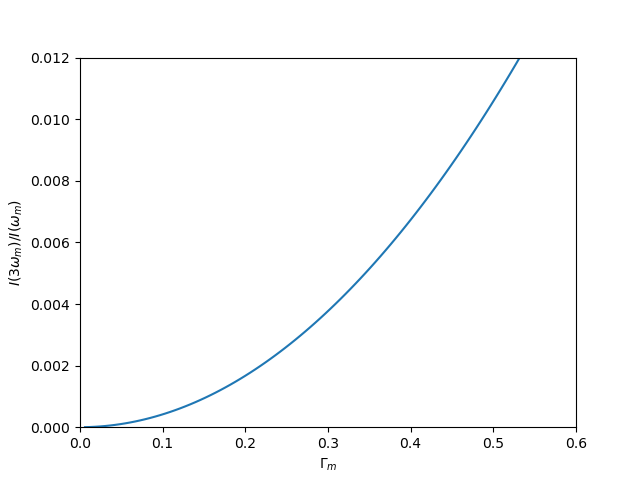
\includegraphics[width=.4\columnwidth]{Figures/14.3-1.png}}
        \subfigure{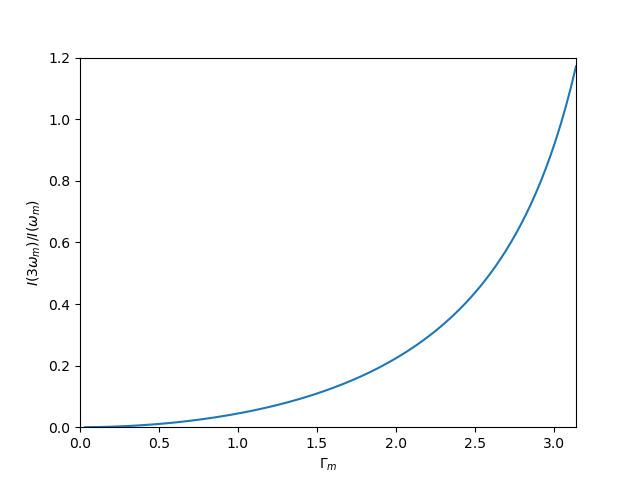
\includegraphics[width=.4\columnwidth]{Figures/14.3-2.png}}
        \caption{出射强度的三次谐波 $(3\omega_m)$ 与基波的比值随 $\Gamma_m$ 的变化曲线.}
        \label{14.3}
    \end{figure}
    由上图知, 若要求该比值不超过 $10^{-2}$, 则最大允许的 $\Gamma_m$ 为 $0.5$.
\end{sol}

\begin{exe}
    试证明, 如一位相调制光波入射在一平方律探测器上, 则输出中只有直流成分.
\end{exe}
\begin{pf}
    相位调制光波的电场矢量可表为如下形式:
    \begin{align}
        E(t)=Ae^{i\phi(t)},
    \end{align}
    故平方率探测器的输出仅有直流成分:
    \begin{align}
        I\propto\abs{E(t)}^2=A^2.
    \end{align}
\end{pf}

\begin{exe}
    利用参考文献 [8] 和 [9], 设计一个在频率 $\nu_m=10^9$ 赫时运转的部分负载 KDP 位相调制器并得到 $\delta=\pi/3$ 峰值位相偏移. 问调制功率是多少?
\end{exe}
\begin{sol}
    如图 \ref{14.5-fig} 所示, 类似文献 \footnote{Peters, C. J. "Gigacycle bandwidth coherent light traveling-wave phase modulator." \itshape{Proceedings of the IEEE} 51.1 (1963): 147-153.} 中提出的行波调制结构, 光沿 KDP 晶体的 $z$ 轴传播, 偏振平行晶体的 $x$ 轴, 在晶体的 $z$ 方向上下安装两片平行于 $xy$ 平面的行波电极, 光波长为 $1\,\mu$m, 晶体宽 $a=1$ mm, 长度 $l=50$ cm, 为了实现外加电场和光场的相位匹配, 电极宽度
    \begin{align}
        w=\frac{a(\epsilon_1-1)}{n_o^2-1}=\frac{1\text{ mm}\times(20.2-1)}{1.5^2-1}=15.6\text{ mm}.
    \end{align}
    为实现电极传输线阻抗与电源阻抗 (通常为 50 $\Omega$) 的匹配, 晶体高度
    \begin{align}
        \notag b=&Z_0\left[\frac{w\epsilon_0(w-a+\epsilon_1a)}{\mu_0}\right]^{1/2}\\
        \notag=&50\,\Omega\left[\frac{15.6\times 10^{-3}\text{ m}\times8.85\times 10^{-12}\text{ F/m}\times(15.6\times 10^{-3}\text{ m}-1\times 10^{-3}\text{ m}+20.2\times 1\times 10^{-3}\text{ m})}{4\pi\times 10^{-7}\text{ F/m}}\right]^{1/2}\\
        =&3.10\text{ mm}.
    \end{align}
    由课本表 14.3, 调制器的相位延迟与调制电压之间的关系为
    \begin{align}
        \Gamma_m=\frac{\pi}{\lambda}\frac{l}{b}n_o^3r_{41}V_m,
    \end{align}
    在相位匹配的条件下, 在频率 $\nu_m=10^9$ Hz 下得到 $\Gamma_m=\delta=\pi/3$ 的峰值相位偏移, 调制电压为
    \begin{align}
        V_m=\frac{\Gamma_m\lambda b}{\pi ln_o^3r_{41}}=\frac{\frac{\pi}{3}\times 1\times 10^{-6}\text{ m}\times 3.10\times 10^{-3}\text{ m}}{\pi\times 0.5\text{ m}\times1.5^3\times 8.47\times 10^{-12}\text{ m/V}}=72.3\text{ V}.
    \end{align}
    调制功率为
    \begin{align}
        P_m=\frac{V_m}{2Z_0^2}=\frac{(72.3\text{ V})^2}{2\times 50\,\Omega}=52.3\text{ W}.
    \end{align}
    \begin{figure}[H]
        \centering
        \subfigure[光学相位调制器示意图.]{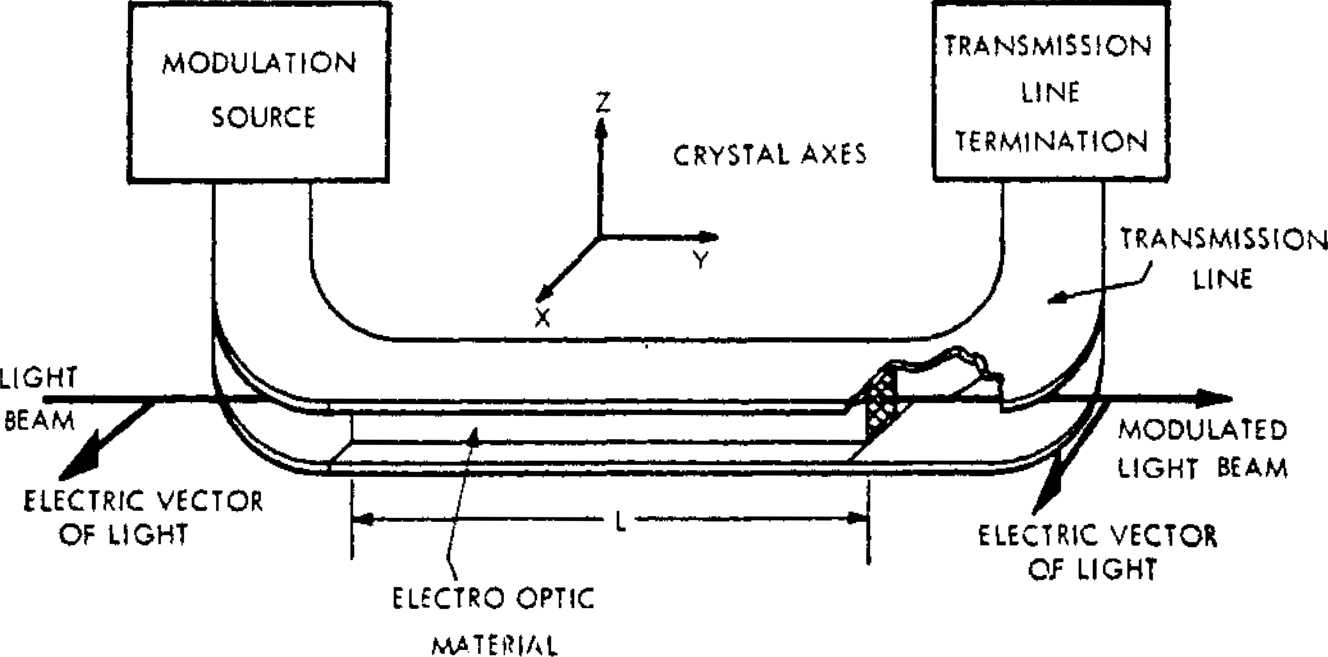
\includegraphics[width=.4\columnwidth]{Figures/14.5-optical-phase-modulator.png}}
        \subfigure[光学相位调制器截面图.]{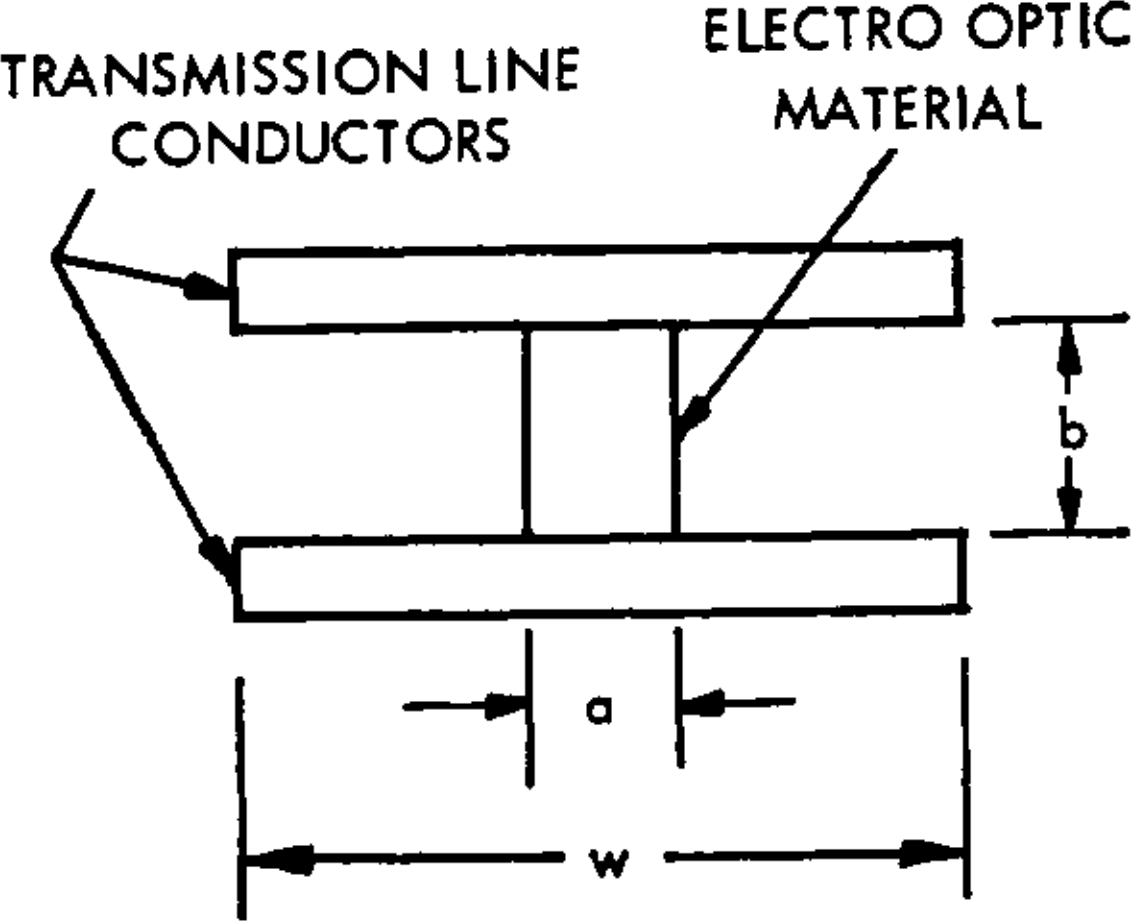
\includegraphics[width=.4\columnwidth]{Figures/14.5-optical-phase-modulator-cross-sectional-view.png}}
        \caption{}
        \label{14.5-fig}
    \end{figure}
\end{sol}

\begin{exe}
    推导型号如 14.5 节举例中所描述的横向 $\bar{4}3m$ 晶体光电调制器的调制功率的表达式 (类似式 (14.6-2)).
\end{exe}
\begin{pf}
    由课本式 (14.5-9), 横向 $\bar{4}3m$ 晶体相位调制器的相位延迟与调制电压之间的关系为
    \begin{gather}
        \Gamma_m=\frac{\sqrt{3}\pi n_o^3r_{41}}{\lambda}\frac{V_ml}{d},\\
        \Longrightarrow V_m=\frac{\Gamma_m\lambda d}{\sqrt{3}\pi n_o^3r_{41}l}.
    \end{gather}
    由课本式 (14.6-1), 极大调制带宽为
    \begin{gather}
        \Delta\nu=\frac{\Delta\omega}{2\pi}\approxeq\frac{1}{2\pi R_LC},\\
        \Longrightarrow R_L=\frac{1}{2\pi C\Delta\nu},
    \end{gather}
    其中调制器电极的电容可用平行板电容的决定式得到:
    \begin{align}
        C=\frac{\varepsilon lw}{d},
    \end{align}
    $l$, $w$ 和 $d$ 分别为晶体的长、宽和高.
    调制器的调制功率为
    \begin{align}
        P=\frac{V_m^2}{2R_L}=\frac{\Gamma_m^2\lambda^2d^2}{6\pi^2n_o^2r_{41}^2l^2R_L}=\frac{\Gamma^2\lambda^2A\varepsilon\Delta\nu}{3\pi n_o^6r_{41}^2l},
    \end{align}
    其中晶体截面积 $A=wd$.
\end{pf}

\begin{exe}
    \begin{itemize}
        \item[(a)] 试证明, 在如图 14.4 装置中光线与 $z$ 轴成 $\theta$($\ll 1$) 的角度传播, 它使双折射对位相延迟的影响为
        \[
            \Delta\Gamma_{\text{双折射}}=\frac{\omega l}{2c}n_o\left(\frac{n_o^2}{n_e^2}-1\right)\theta^2.
        \]
        相应的折射率变化为
        \[
            n_o-n_e(\theta)=\frac{n_o\theta^2}{2}\left(\frac{n_o^2}{n_e^2}-1\right).
        \]
        \item[(b)] 导出最大允许束散角的近似表达式, 在此束散角下 $\Delta\Gamma_{\text{双折射}}$ 并不妨碍调制器的运转.
    \end{itemize}
    答案:
    \[
        \theta<\left[\frac{\lambda}{4n_ol\left(\frac{n_o^2}{n_e^2}-1\right)}\right]^{1/2}.
    \]
\end{exe}
\begin{sol}
    \begin{itemize}
        \item[(a)] 当光线与 $z$ 轴成 $\theta$ ($\ll 1$) 的角度传播时, o 光的折射率仍为 $n_o$, e 光的折射率为
        \begin{align}
            \frac{1}{n_e^2(\theta)}=\frac{\cos^2\theta}{n_o^2}+\frac{\sin^2\theta}{n_e^2},
        \end{align}
        \begin{align}
            \Longrightarrow n_e(\theta)=&\left(\frac{\cos^2\theta}{n_o^2}+\frac{\sin^2\theta}{n_e^2}\right)^{-1/2}=\left(\frac{1}{n_o^2}+\frac{n_o^2-n_e^2}{n_o^2n_e^2}\sin^2\theta\right)^{-1/2}=n_o\left(1+\frac{n_o^2-n_e^2}{n_e^2}\sin^2\theta\right)^{-1/2}\\
            \approx&n_o\left(1+\frac{n_o^2-n_e^2}{2n_e^2}\sin^2\theta\right)\approx n_o\left(1+\frac{n_o^2-n_e^2}{n_e^2}\theta^2\right).
        \end{align}
        o 光与 e 光的折射率差为
        \begin{align}
            n_o-n_e(\theta)=\frac{n_o\theta^2}{2}\left(\frac{n_o^2}{n_e^2}-1\right).
        \end{align}
        该折射率差产生的双折射相对相位延迟为
        \begin{align}
            \Delta\Gamma_{\text{双折射}}=kl[n_o-n_e(\theta)]=\frac{\omega l}{2c}n_o\left(\frac{n_o^2}{n_e^2}-1\right)\theta^2.
        \end{align}
        \item[(b)] 要使 $\Delta\Gamma$ 不妨碍调制器的运转, 即
        \begin{align}
            \Delta\Gamma_{\text{双折射}}=\frac{\omega l}{2c}n_o\left(\frac{n_o^2}{n_c^2}-1\right)\theta^2<\frac{\pi}{4},
        \end{align}
        则最大允许散射角
        \begin{align}
            \theta<\left[\frac{\lambda}{4n_ol\left(\frac{n_o^2}{n_e^2}-1\right)}\right]^{1/2}.
        \end{align}
    \end{itemize}
\end{sol}

\begin{exe}
    查阅文献 (例如可阅读文献 [17] 和 [18]) 并阐述布拉格衍射和德拜-西尔斯 (Debye-Sears) 衍射之间的差别. 在什么条件下可观察到每种衍射?
\end{exe}
\begin{sol}
    德拜-西尔斯衍射: 如图 \ref{14.8-fig}(a)(b) 所示, 入射光 (频率为 $\omega$, 波长为 $\lambda$, 波矢为 $\bm{\beta}$) 传播方向与声波 (频率为 $\omega_m$, 波长为 $\Lambda$, 波矢为 $\bm{k}_s$) 传播方向垂直, 产生频率分别为 $\omega\pm\omega_m$, $\omega\pm 2\omega_m$, $\omega\pm 3\omega_m$, $\cdots$ 等一系列边带的衍射光, 分别与原入射方向成夹角 $\pm\arcsin\frac{\lambda}{\Lambda}$, $\pm\arcsin\frac{2\lambda}{\Lambda}$, $\pm\arcsin\frac{3\lambda}{\Lambda}$, $\cdots$ 出射. 如图 \ref{14.8-fig}(c) 所示, 各级次的衍射光的振幅与声波调制引起的相位变化幅度 $\Delta\phi=2\pi\frac{l}{\lambda}\Delta n$ 有关.

    布拉格衍射的条件: 除了要求出射光频率 $\omega'=\omega\pm\omega_m$, $\omega\pm 2\omega_m$, $\omega$, 波矢 $\bm{\beta}'=\bm{\beta}\pm\bm{k}_s$, $\bm{\beta}\pm 2\bm{k}_s$, $\bm{\beta}\pm 3\bm{k}_s$, $\cdots$, 还需材料厚度 $l$ 满足 $2\pi\lambda l\ll\Lambda^2$.

    布拉格衍射: 如图 \ref{14.8-fig}(d) 所示, 入射光传播方向与声波波前平面成夹角 $\frac{\lambda}{2\Lambda}$, 产生频率为 $\omega+\omega_m$, 传播方向与声波波前成夹角 $-\frac{\lambda}{2\Lambda}$ 的衍射光. 布拉格衍射对衍射级次的选择性很强, 其余边带由于相干相消的效应被抑制, 因而只有一个频率分量的衍射光出射.

    布拉格衍射的条件为: 出射光频率 $\omega'=\omega\pm\omega_m$, 波矢 $\bm{\beta}'=\bm{\beta}\pm\bm{k}_s$ ($\pm$ 取决于声波的方向), 对材料厚度无要求.

    \footnote{参考文献: Adler, Robert. "Interaction between light and sound." \itshape{IEEE spectrum} 4.5 (1967): 42-54.}
    \begin{figure}[H]
        \centering
        \subfigure[德拜-西尔斯衍射, 入射光正入射介质, 声波传播方向与入射光传播方向垂直, 声波在介质中形成周期性压缩和拉伸的密度分布, 载波频率 (入射光频率) 的出射光沿原有传播方向出射, 一阶上边带 (频率为载波频率与一倍声波频率的和) 的衍射光与原有传播方向成夹角 $\frac{\lambda}{\Lambda}$ 出射, 其余频率和出射方向的衍射光未画出.]{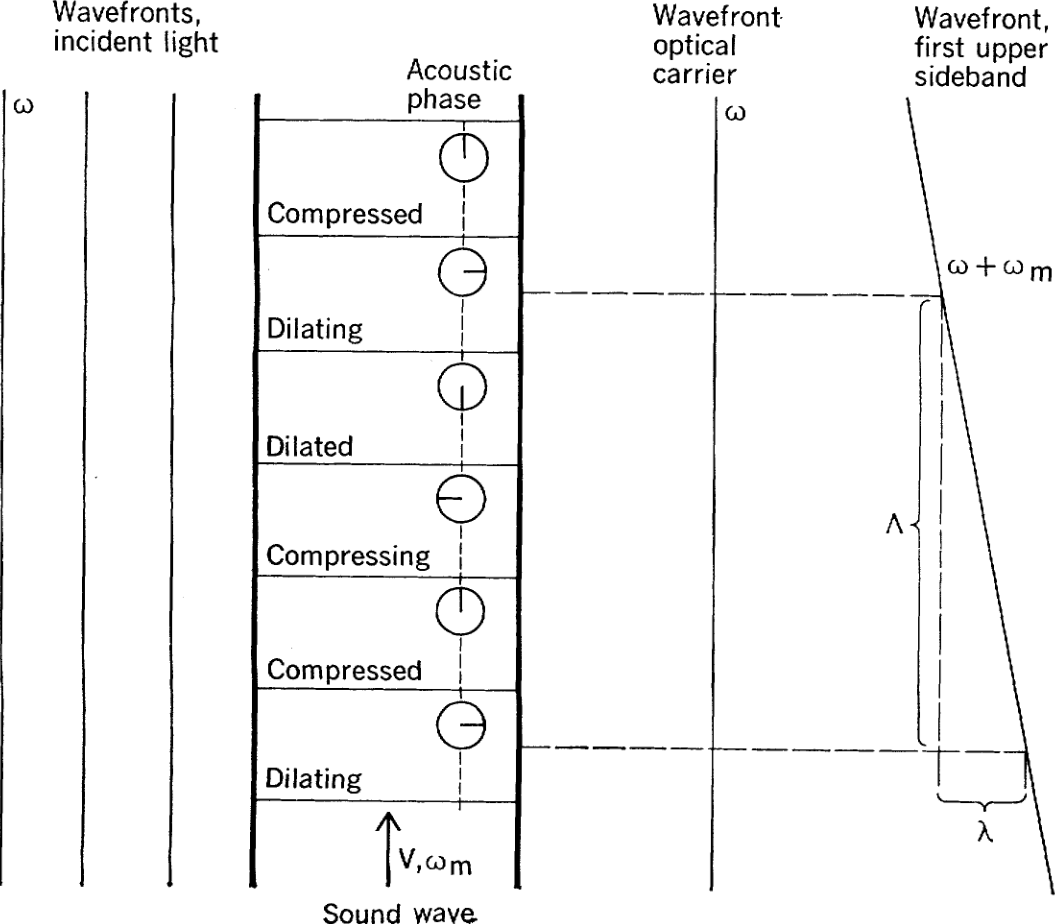
\includegraphics[width=.4\columnwidth]{Figures/14.8-Debye-Sears-diffraction.png}}
        \subfigure[德拜-西尔斯衍射载频和边带频谱.]{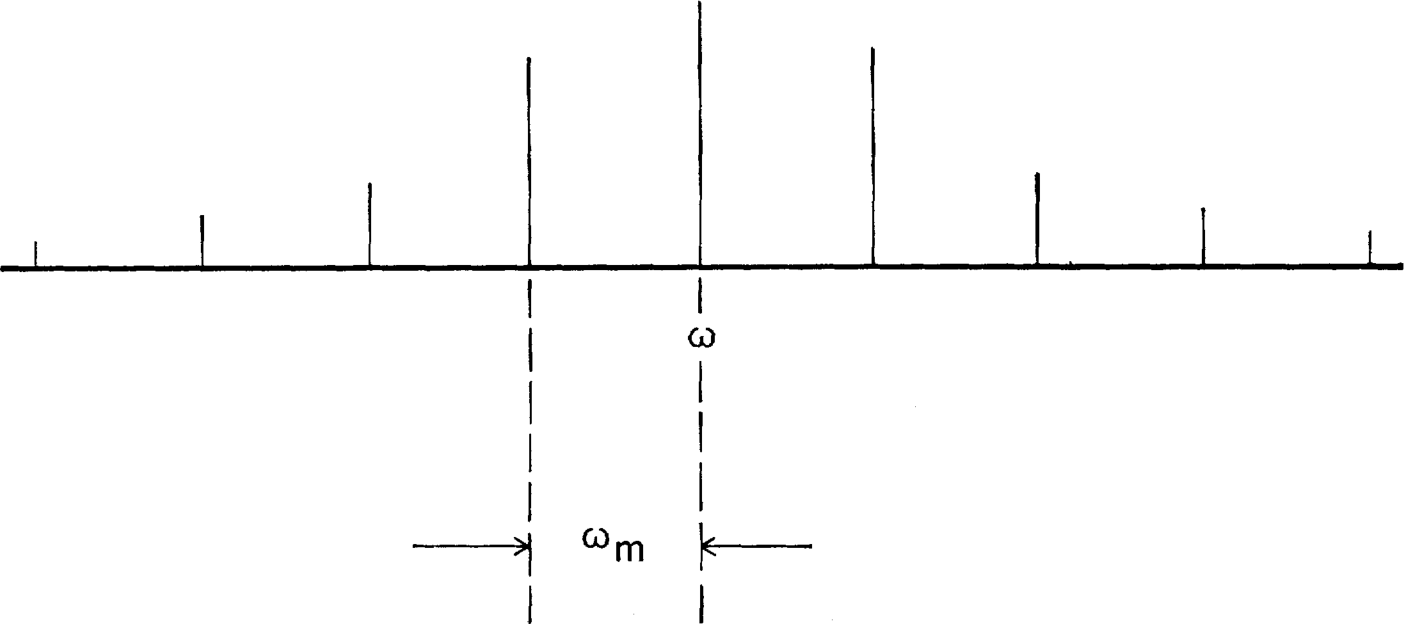
\includegraphics[width=.4\columnwidth]{Figures/14.8-Bragg-diffraction-side-band.png}}
        \subfigure[德拜-西尔斯衍射载频及各边带出射光归一化振幅与声致相位差幅值的关系, 这些曲线即为各阶 Bessel 函数.]{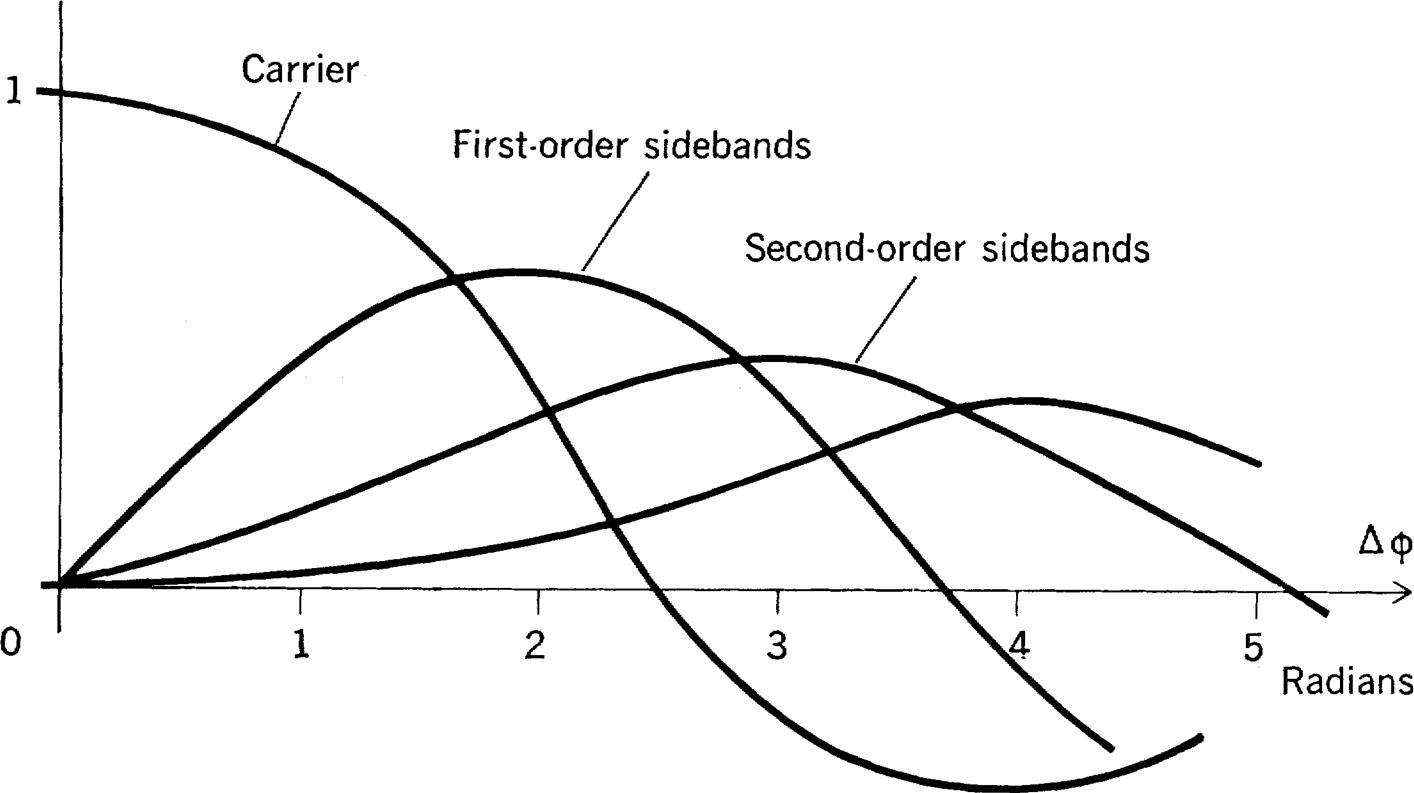
\includegraphics[width=.4\columnwidth]{Figures/14.8-Bragg-diffraction-side-band-amplitude.png}}
        \subfigure[布拉格衍射.]{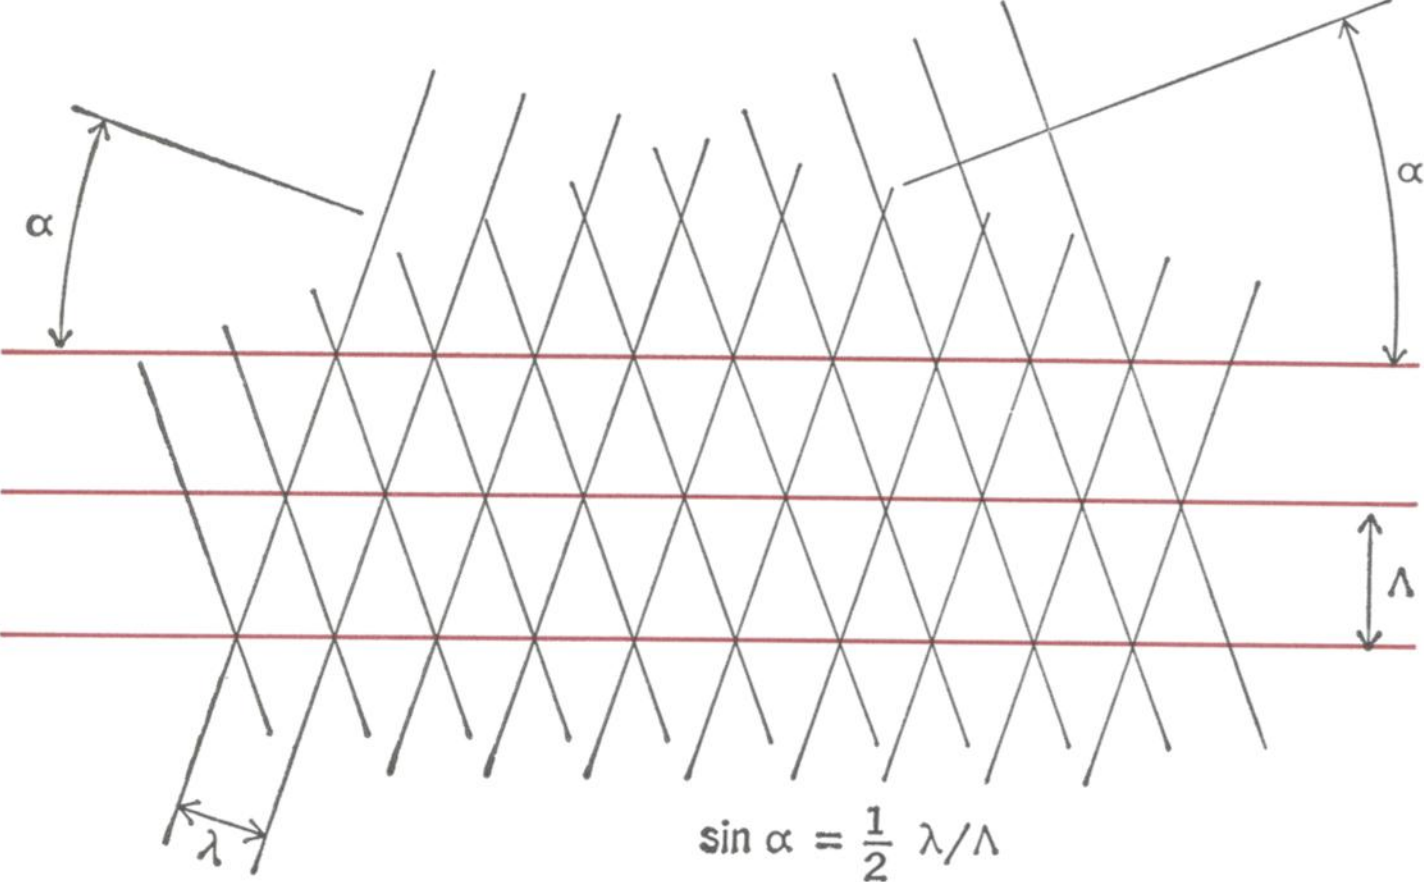
\includegraphics[width=.4\columnwidth]{Figures/14.8-Bragg-diffraction.png}}
        \caption{}
        \label{14.8-fig}
    \end{figure}
\end{sol}

\begin{exe}
    晶体中 $X$ 射线衍射的布拉格定律为
    \[
        2d\sin\theta=m\frac{\lambda}{n},\quad m=1,2,3
    \]
    式中 $n$ 为折射率, $d$ 为等价原子平面间的距离, $\theta$ 为入射角, 而 $\lambda$ 为衍射辐射在真空中的波长. 当 $2\lambda_s\sin\theta=\frac{\lambda}{n}$ 时光与声波作用而产生布拉格衍射 (参见图 14.15). 与 X 射线衍射结果相比较并取 $\lambda_s=d$, 则只有 $m=1$ 的情况是允许的. 解释其差别. 对于受声波散射的情况, 为什么不能得到对应于 $m=2,3,\cdots$ 的衍射角 $\theta$ 呢?\\
    提示: X 射线衍射发生在分立的原子平面上, 它可被理想化为无限薄的薄片, 而声波的扰动则是正弦曲线的.
\end{exe}
\begin{sol}
    当 X 射线受声波散射时, 由于声波
    \begin{align}
        S_{kl}(\bm{r},t)=\frac{S_{kl}}{2}e^{i(\omega_st-\bm{k}\cdot\bm{r})}+\text{c.c.}
    \end{align}
    仅有一个频率为 $\pm\omega_s$ 的分量, 故其引起的电极化强度扰动
    \begin{align}
        \Delta P_i(\bm{r},t)=-\frac{1}{4}\varepsilon_0\varepsilon_i'\varepsilon_d'p_{idkl}E_d(r_d)[e^{i(\omega_dt-\bm{k}_d\cdot\bm{r})}+\text{c.c.}]\times S_{kl}[e^{i(\omega_st-\bm{k}_s\cdot\bm{r})}+\text{c.c.}],
    \end{align}
    仅有频率为 $\pm(\omega_d+\omega_s)$ 和 $\pm(\omega_d-\omega_s)$ 的分量, 故仅在
    \begin{align}
        \omega_i=&\omega_d\pm\omega_s,\\
        \bm{k}_i=&\bm{k}_d\pm\bm{k}_s
    \end{align}
    下能满足能量守恒和动量守恒.

    而当 X 受晶格散射时, 由于周期性排布的原子平面引起的扰动包含等频率间隔的多个分量:
    \begin{align}
        A_{kl}(\bm{r})=\sum_{m=0}^{\infty}A_{kl}(m\omega_a)e^{im(\omega_a-\bm{k}_at)}+\text{c.c.}
    \end{align}
    故其引起的电极化强度扰动
    \begin{align}
        \Delta P_i\propto E_d(\bm{r},t)A_{kl}(\bm{r},t)=E_d(r_d)[e^{i(\omega_dt-\bm{k}_d\cdot\bm{r})}+\text{c.c.}]\times\left[\sum_{m=0}^{\infty}A_{kl}(m\omega_a)e^{im(\omega_a-\bm{k}_at)}+\text{c.c.}\right]
    \end{align}
    有频率为 $\pm(\omega_d\pm m\omega_a)$ 的多个分量, 故在
    \begin{align}
        \omega_i=&\omega_d\pm m\omega_a,\\
        \bm{k}_i=&\bm{k}_d\pm m\bm{k}_a,\quad m=1,2,3,\cdots
    \end{align}
    下均能满足能量守恒和动量守恒.
\end{sol}

\begin{exe}
    对 $\Delta k=\abs{\bm{k}_i-\bm{k}_s-\bm{k}_d}\neq 0$ 和小输入信号 $E_i(0)$ 的情况, 解耦合模方程 (14.9-8). 假设有共线相互作用, 则 $r_i=r_d=r_s=z$. 试证明入射功率转化为衍射光束的最大比率为
    \[
        \frac{\eta^2}{\eta^2+\left(\frac{\Delta k}{2}\right)^2}.
    \]
    可见, 可允许的失配量 $\Delta k$ 同 $\eta$ 有关. 你能对违反动量守恒作出直观的解释吗?
\end{exe}
\begin{pf}
    对 $\Delta k=\abs{\bm{k}_i-\abs{\bm{k}_s}-\bm{k}_d}\neq 0$、小输入信号 $E_i(0)$ 且共线情况下, 耦合模方程 (14.9-8) 可写为
    \begin{align}
        \label{14.10-1}
        \frac{\mathrm{d}E_i}{\mathrm{d}z}=&i\eta E_de^{i\Delta kz},\\
        \label{14.10-2}
        \frac{\mathrm{d}E_d}{\mathrm{d}z}=&i\eta E_ie^{-i\Delta kz},
    \end{align}
    其中 $\eta\equiv\eta_{di}=\eta_{id}\approxeq\frac{\pi n^3}{2\pi}p_{idkl}S_{kl}$.
    对式 \eqref{14.10-1} 关于 $z$ 求偏导并利用式 \eqref{14.10-2} 和 \eqref{14.10-2} 消去 $E_d$ 得
    \begin{align}
        \frac{\mathrm{d}^2E_i}{\mathrm{d}z^2}-i\Delta k\frac{\mathrm{d}E_i}{\mathrm{d}z}+\eta^2E_i=0,
    \end{align}
    结合初始条件 $E_i(0)$ 和 $\frac{\mathrm{d}E_i}{\mathrm{d}z}(0)=i\eta E_d(0)$ 解得
    \begin{align}
        E_i(z)=&\left[E_i(0)\cos\left(\frac{\sqrt{\Delta k^2+4\eta^2}}{2}z\right)+i\frac{-\Delta kE_i(0)+2\eta E_d(0)}{\sqrt{\Delta k^2+4\eta^2}}\sin\left(\frac{\sqrt{\Delta k^2+4\eta^2}}{2}z\right)\right]e^{i\Delta kz/2}.
    \end{align}
    在小输入信号情况下, $E_i(0)\ll E_d(0)$, 故入射功率转化为衍射光束的最大比率为
    \begin{align}
        \frac{\abs{E_i(z)}^2}{\abs{E_d(0)}^2}=\frac{\abs{E_i(0)}^2+\abs{\frac{-\Delta kE_i(0)+2\eta E_d(0)}{\sqrt{\Delta k^2+4\eta^2}}}^2}{\abs{E_d(0)}^2}\approx\frac{\eta}{\sqrt{\eta^2+\left(\frac{\Delta k^2}{2}\right)^2}}.
    \end{align}
\end{pf}% TODO

\begin{exe}
    从多普勒理论和式 (14.9-12) 推导出式 (14.9-11).
\end{exe}
\begin{pf}
    将声波视为以声速传播的周期性晶格.
    以声波为参考系, 由相对论多普勒效应, 入射光的频率为
    \begin{align}
        \omega_i'=\frac{\omega_i}{\left(1-\frac{nv}{c}\sin\theta\right)\sqrt{1-\frac{n^2v^2}{c^2}}},
    \end{align}
    在声波参考系中, 声波静止, 故散射光的频率等于入射光的频率
    \begin{align}
        \omega_s'=\omega_i'.
    \end{align}
    在实验室参考系中, 散射光的频率为
    \begin{align}
        \omega_s=\frac{\omega_s'}{\left(1-\frac{nv}{c}\sin\theta\right)\sqrt{1-\frac{n^2v^2}{c^2}}}=\frac{\omega_i}{\left(1-\frac{nv}{c}\sin\theta\right)^2\left(1-\frac{n^2v^2}{c^2}\right)},
    \end{align}
    由于声速 $v\ll$ 光速 $c$, 故有近似
    \begin{align}
        \label{14.11-1}
        \omega_d\approx\omega_i\left(1+\frac{2nv}{c}\sin\theta\right).
    \end{align}
    式 (14.9-12) 描述了光波长和声波长之间的关系:
    \begin{align}
        2\lambda_s\sin\theta=\frac{\lambda}{n},
    \end{align}
    其中声波长 $\lambda_s=\frac{2\pi v}{\omega_s}$, 光波长 $\lambda=\frac{2\pi c}{\omega_i}$, 故由上式得
    \begin{align}
        \sin\theta=\frac{\omega_sc}{2n\omega_iv}.
    \end{align}
    将上式代入式 \eqref{14.11-1} 中得
    \begin{align}
        \omega_d=\omega_i+\omega_s.
    \end{align}
\end{pf}
\ifx\allfiles\undefined
\end{document}
\fi